\chapter{Introducción específica} % Main chapter title

\label{Chapter2}

En el presente capítulo se introducen las tecnologías y herramientas de hardware y software en todos los niveles utilizados en el desarrollo del trabajo. 

\section{Protocolos de comunicación}
\subsection{Modelo OSI}

El modelo de interconexión de sistemas abiertos, conocido como modelo OSI, (en inglés, \textit{Open Systems Interconnection}) es un modelo de referencia para los protocolos de la red. Define un estándar que tiene por objetivo interconectar sistemas de procedencia distinta para que estos puedan intercambiar información sin ningún tipo de impedimentos. Está conformado por 7 capas o niveles de abstracción. Cada uno de estos niveles tiene sus propias funciones para que en conjunto sean capaces de poder alcanzar su objetivo final. Precisamente esta separación en niveles hace posible la intercomunicación de protocolos distintos al concentrar funciones específicas en cada nivel de operación. \citep{8}

\begin{figure}[h]
\centering
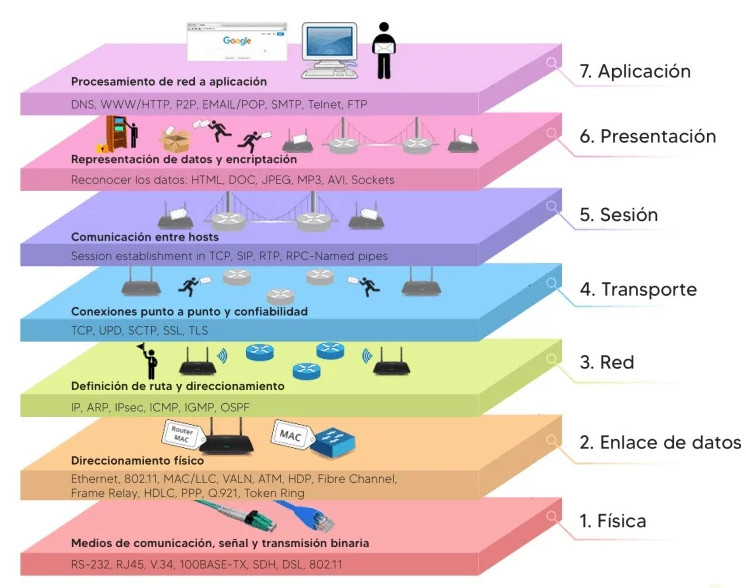
\includegraphics[scale=0.43]{Imagen 4 - Modelo OSI.jpg}
\caption[Modelo OSI]{Modelo OSI. \footnotemark}
\label{fig:4}
\end{figure}
\footnotetext{Imagen tomada de: \url{https://platzi.com/clases/2225-redes/35587-modelo-osi/}}

\subsection{Enlace Wi-Fi y ethernet}



\subsection{Protocolo HTTP}



\subsection{Protocolo MQTT}